\documentclass[letterpaper,12pt,twocolumn]{article}
\pagestyle{empty}

\pdfpagewidth 8.5in
\pdfpageheight 11in

\hoffset = 0pt
\oddsidemargin = 0pt
\marginparwidth = 0pt

\voffset = 0pt
\topmargin = 0pt
\headheight = 0pt
\headsep = 12pt

\textwidth = 7in
\textheight = 9.5in
\footskip = 0pt

\usepackage{amsmath}
\usepackage{amssymb}
\usepackage{hyperref}
\usepackage{graphicx}

\author{Erik Keever}
\title{Radiating Shock experiment documentation}

\begin{document} 

\maketitle

\section{Overview}

The radiating shock experiment generates equilibrium solutions of the one 
dimensional equations of radiating hydrodynamic or ideal magnetohydrodynamic flows
and runs them with a small seed perturbation immediately upstream of the shock front.

\section{Equilibrium conditions}

To begin with we state the equations of Ideal MHD with a polytropic equation of state,

\begin{subequations} \label{fulleqns}
\begin{align}
\partial_t \rho &+  \nabla (\rho v) &= 0 \\
\partial_t (\rho \mathbf{v}) &+ \nabla (\rho \mathbf{v} \mathbf{v} + \mathbf{I} P - B B) &= 0 \\
\partial_t B &+ \nabla (v B - B v) &= 0 \\
\partial_t E &+ \nabla (\mathbf{v}(E+P) - (\mathbf{v} \cdot \mathbf{B})\mathbf{B} ) &= 0
\end{align}
\end{subequations}

Where we define $\rho$ as the matter density, $\mathbf{v}$ its velocity, $P$ the total (gas plus magnetic) pressure, $\mathbf{I}$ the identity tensor and $\mathbf{B}$ the magnetic field (with $\mu_0 = 1$).

Assuming an equilibrium solution ($\partial_t \rightarrow 0$), that we have structure 
only in the x direction ($\partial_y = \partial_z \rightarrow 0$), and that we have 
entered the deHoffman-Teller frame ($\vec{v} || \vec{B})$, a 
series of conserved quantities associated with the above system (now a set of coupled ODEs) 
now clearly arises by going to the integral form: The derivatives of the fluxes are zero
so the fluxes themselves must be constants.

\begin{subequations} \label{invariants}
\begin{align}
p_x &= \rho_0 vx_0 \\
f_x &= \rho_0 vx_0^2 + P_0 - Bx_0^2 \\
f_y &= \rho vx_0 vy_0 - bx_0 by_0 \\
0 &= vx_0 by_0 - bx_0 vy_0 \\
bx &= bx_0 \\
E_0 &= \frac{\rho v^2}{2} + \frac{\gamma P}{\gamma-1} - b_x \mathbf{v} \cdot \mathbf{B}
\end{align}
\end{subequations}

This is of course a restatement of the Rankine-Hugoniot conditions of an ideal MHD
flow. There nominally exist terms in the z direction as well. However, shock solutions 
do not change the vector angle $\tan(\phi) = bz/by = vz/vy$ so we implicitly 
assume this symmetry and work in the X-Y plane only.

The RH equations define the entire standing 1D shock flow assuming any 6 things are known.
In the standard view, we presume to know the upstream conditions and then solve exactly
for the downstream conditions. This results in a fourth degree polynomial in the final
variable.

If the flow were adiabatic, the solution of the quartic and selection of the correct
root would be the end of it.
However we let there exist a radiation function $\Gamma(\rho, P)$ which breaks the
conservation of energy flux.

Choosing $vx$ as the variable, we may use \ref{invariants}.a-\ref{invariants}.d to 
solve for $\rho$, $vy$, $by$ and $P_{gas}$ in terms of the invariants and vx only:

\begin{subequations}
\begin{align}
\rho = p_x / vx \\
vy = f_y bx_0 / (p_x vx - bx_0^2) \\
by = bx_0 f_y / (p_x vx - bx_0^2) \\
P_{gas} = f_x - p_x vx + (bx_0^2 - by(vx)^2)/2
\end{align}
\end{subequations}

There is now just one nonlinear ODE to solve numerically. It is formulated by

\begin{equation}
\partial_{vx} (\text{\ref{fulleqns}.d}) \partial_x vx = -\Gamma(\rho, P)
\end{equation}

None of equations (\ref{fulleqns}) depend on x explicitly (as we would certainly
expect of Galilean-invariant things) so we use the chain rule to get an equation
in terms of $x$.

By electing that $vx$ be a parameterized trial function of $x$, the system may be
solved numerically by any desired ODE solver as accurately as desired.

\section{Numeric Solution}

The Taylor series always (mathematically) works at any ordinary point of an ODE.
Imogen's RadiatingFlowSolver contains the first 4 terms for the MHD case and the first
6 terms for the hydrodynamic case. The use of Pade approximant transforms is found to
considerably improve the convergence properties of the series.

However, the direct series expansions are unwieldy (the 4th MHD term took 4 hours for
Mathematica to simplify and is still over 2000 characters long) and contain so many terms
that even evaluating them numerically is no longer a trivially foregone conclusion.

Imogen's solver therefore by default only uses them to generate past-history points 
to initialize a linear multistep method (See the .solver() method), which may be
either 5th order explicit (AB5), or 6th (AM5) or 7th (AM6) order implicit.

\subsection{Hydrodynamic endpoint}

There are three possible outcomes in the general integration case. If it is 
hydrodynamic ($\mathbf{B} = \mathbf{0}$) with $\theta > -3$, 
the solution reaches zero velocity / infinite density in a finite distance; the
velocity curve approaches this point with infinite derivative. The numerical solver
adapts by sharp curvature by reducing step size; It is given only a finite number of
adapts before terminating and typically follows the solution to a vx of 1/10000 the
original value.

\subsection{Thermal cutoff}

Normally a temperature cutoff is imposed on the radiation, such that
$\Gamma(T < T_{crit}) \rightarrow 0$ which makes the flow revert to adiabatic
(uniform flow) behavior thereafter. $v_{\text{terminal}}$ is given by solving the
quadratic (HD) or quartic (MHD) polynomial $P_{gas}/\rho = T_{crit}$ for $vx$.
In the hydrodynamic case the answer is
\[ v_{\text{terminal}} = (f_p - \sqrt{f_p^2 - 4 p_x^2 T_{\text{crit}} })/ 2 p_x \]
with momentum flux $f_p$, momentum $p_x$ and cutoff $T_{\text{crit}}$, where
subtracting the discriminant gives the physical (terminal velocity is lower)
solution. It can be seen that this reduces to a terminal velocity of zero if 
the temperature cutoff is zero.

The MHD flow's velocity at temperature cutoff is the largest magnitude of the polynomial P,
\begin{eqnarray}
c_4 &= -2 p_x^3 \\
c_3 &= p_x^2 (2 f_p + 5 B_x^2) \\
c_2 &= p_x (-4 B_x^4 - 4 B_x^2 f_p - 2 p_x^2 T_\text{crit}) \\
c_1 &= B_x^2 (B_x^4 + 2 B_x^2 f_p - f_y^2 + 4 p_x^2 T_\text{crit}) \\
c_0 &= -2 B_x^4 p_x T_\text{crit} \\
P(v_x) &= \displaystyle\sum_{i=0}^4 c_i v_x^i 
\end{eqnarray}
which is of the same sign and smaller magnitude than the initial velocity. As the magnetic
field becomes weak two of the roots become degenerate at $x=0$ and the original
quadratic is recovered.

\subsection{Magnetic support}

A alternate scenario for magnetized flows which pure fluids do not have is a
transition to purely magnetic support, i.e. the flow can continue forever in space. When
the flow becomes low-$\beta$ the flow parameters abruptly rearrange themselves,
with the sudden collapse of pressure and equally abrupt increase in $B_y$ as
depicted in figure 1. 

\begin{figure*}
\title{Radiating MHD flow near knee}
\centering 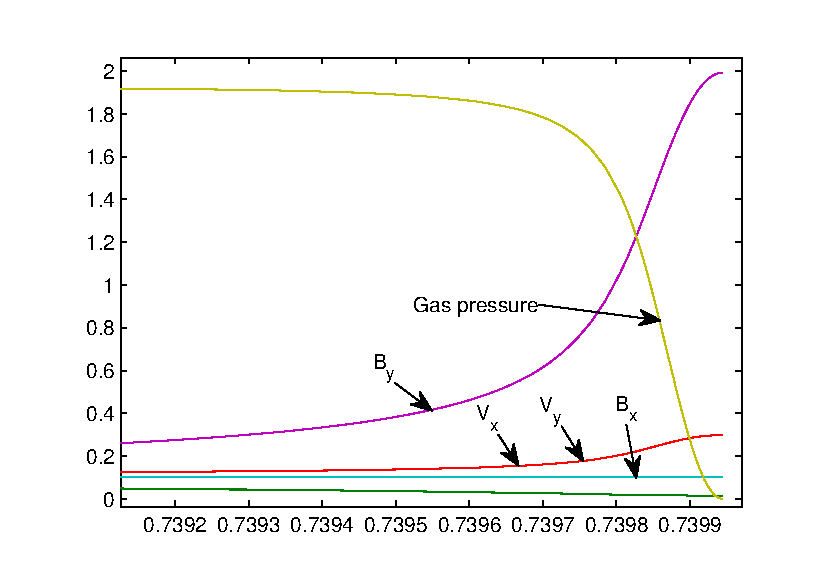
\includegraphics{bsupport}
\caption{As the plasma beta drops past 1 the flow parameters almost instantly
change. Sample initial parameters were $\rho = v_x = P = 1$, $v_y = b_x = .1$, $b_y = .01$, $\gamma=5/3$, $\beta_{rad} = 1$, $\theta_{rad} = .5$ } \label{kneefig}
\end{figure*}

\subsection{Summary}

RadiatingFlowSolver allows the user to select no cutoff, magnetization cutoff times
a value slightly greater than unity, or thermal cutoff with arbitrary temperature
ratio (selecting a low thermal cutoff for a magnetized flow approaches the 
magnetization cutoff itself).

The integrator itself actually terminates on one of three conditions:
\begin{itemize}
\item Too many restarts - Every time a physically invalid $vx$ occurs, the 
engine backs up, reduces the space step, and resumes. This is only
allowed to happen a certain number of times.
\item Too many steps - A hard cutoff of 20K solver iterations is imposed
\item Reaching the cutoff condition
\end{itemize}

\subsection{Assumptions}

The RadiatingShock experiment's flow solver assumes that the radiation function
is parameterized in the form of
\begin{equation}
\Lambda(\rho, P) = \beta \rho^{2-\theta} P^{\theta}
\end{equation}
I.e. a standard power law radiation model. $\theta = 1/2$ corresponds to free-free
scattering/Bremsstrahlung. However, the accompanying Mathematica notebooks themselves
contain a line which replaces this with a stub for an arbitrary $\Lambda$ (though
the expressions for velocity will, of course, become even more complex).

The assumption of a polytropic equation of state is built into the energy flux
function used to derive all the equations used by the equilibrim solver; Relaxing it
in the derivation notebooks would require rewriting equation 4 in them.

\newpage
\section{Files}

Files involved with this experiment include:

\begin{itemize}
\item run/run\_RadiatingHydroShock.m
\item experiment/RadiatingShock/*
\item experiment/experimentUtils/RadiatingFlowSolver.m
\item experiment/experimentUtils/pade.m
\item experiment/experimentUtils/solveCubic.m
\item experiment/experimentUtils/solveQuartic.m
\end{itemize}

\section{Simulation Parameters}

Physical parameters relevant to the simulation class are:
\begin{itemize}
\item .gamma (5/3) - Set the polytropic index $\gamma$.
\item .fractionPreshock (1/4) - This fraction with the lowest X values starts in uniform adiabatic preshock flow
\item .fractionCold (1/10) - This fraction of the highest X values which start in the condition the flow had when the integrator terminated.
\item .Tcutoff (1) - HACK
\item .theta  (0) - Sets the inclination of the preshock flow to the shock normal
\item .sonicMach (3) - Sets the ratio of X velocity to preshock adiabatic soundspeed
\item .alfvenMach (-1) - Sets the ratio of X velocity to preshock Alfven speed. If less than 0, a hydrodynamic flow is set up.
\item .radBeta (1) - Sets the radiation parameter $\beta$ in $\Lambda = \beta \rho^{2-\theta} P^\theta$
\item .radTheta (1/2) - Sets the $\theta$ parameter in the $\Lambda$ equation above.
\end{itemize}

Numerical parameters of note include:
\begin{itemize}
\item .perturbationType - must be one of .RANDOM (white noise), .COSINE (y-plane monochromatic), .COSINE\_2D (yz-plane monochromatic) to select the type of perturbation used to seed instability
\item .seedAmplitude (5e-4) - Sets the magnitude of the sinusoid or of all Fourier 
coefficients used to generate white noise in the density right upstream of the shock
\item .randomSeed\_spectrumLimit (64) - Cuts off the white noise spectrum at this wavenumber.
\end{itemize}

Note that slow MHD shocks are almost unconditionally unstable to the corrugation
instability; It will exhibit itself in around 20-40K timesteps at cfl=.35 even if the
initial perturbation has amplitude of one part in a billion.

\section{Analysis}

The RHD\_Analyzer() class provides for simple analysis and size-reduction of the data
that results from radiating flow simulations.

It provides the following output results:
\begin{itemize}
\item .frontX(t, x, y): The exact position of the shock surface in grid coordinates,
here defined as where a piecewise linear interpolation in the x direction passes through
the mean of the adiabatic pre- and postshock densities.
\item rhobar(t, x): Average density at a given time/x position; Useful for waterfall plots
\item rmsdrho(t, x): RMS disturbance in density
\item Pbar(t, x): Average pressure
\item rmsdP(t, x): RMS disturbance in pressure
\item vxbar(t, x)
\item vybar(t, x)
\end{itemize}

The analyzer class also has a convenient .generatePlots() method to throw up
images of most of the previous values.

In addition (though this ought be a separate function) generatePlots() will
try to fit an exponential sinusoid to the average shock position fluctuation using
Matlab's lsqcurvefit function.

\end{document}
